During the training phase, the model is evaluated at each epoch on the same set
of validation data. However, this set is made of semi-synthetic image samples,
generated in the same way as for the training set. Even though they are
generated independently, and are very unlikely to comprise identical samples,
they still do not reflect the real target data (as demonstrated in section
\ref{section-realism}).\\


To obtain performance metrics on the authentic gates, a real-world test dataset
is captured by manually flying the drone through physical gates (see
figure~\ref{fig:mygates}), for around five minutes, which produces close to
$8,000$ frames.

In order to annotate this test set, the gate positions and orientations are
recorded using the motion capture system and a hand-held tracker. This pose
information being absolute and fixed, it is then projected onto the image
, for each frame of the dataset. This process can be easily achieved using the
very same technique utilized for the synthetic gates: the absolute position of
the physical obstacles relate to the virtual scene, and the projection is
therefore supposed to work for that case as well.

Furthermore, it is not trivial to automatically select the closest gate to the
camera, while making sure that its center is in the field of view. Due to a
lack of time to implement this feature, every gate in the image frame is
considered a possible candidate. This does not impact the testing in a bad way,
and gives the benefice of the doubt to the predictions that target the wrong
gate.\\

Nevertheless, results showed that this hypothesis might not be in perfect
conditions for the projection to work. Either due to the slight jitter in the
motion capture recordings of the drone, or because of other sources of error,
the projected gate center coordinates end up being shifted on the image.

\begin{figure}[h]
	\centering
	\begin{subfigure}{0.49\textwidth}
		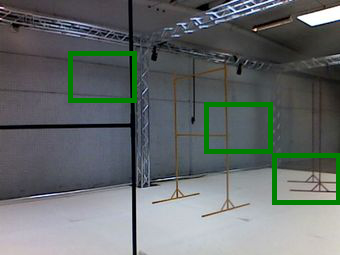
\includegraphics[width=\textwidth]{figure/shifted_gt.png}
		\caption{Shifted ground truth on the test dataset.}
		\label{fig:bad-gt}
	\end{subfigure}
	\begin{subfigure}{0.49\textwidth}
		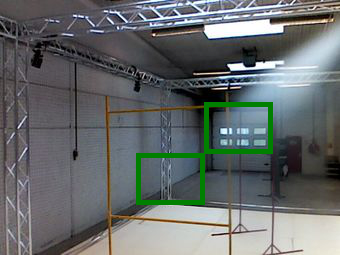
\includegraphics[width=\textwidth]{figure/good_gt.png}
		\caption{Proper ground truth on the test dataset.}
		\label{fig:good-gt}
	\end{subfigure}
	\caption[Shifted and proper ground truth projection]{}
\end{figure}

This discrepancy can grow big enough, in some cases, that the annotations of
the test dataset become unusable (see figure~\ref{fig:bad-gt}). To evaluate the
model's performance on images of real gates, a video is generated from the
ordered sequence of test images where predictions have been annotated as visual
clues. This method allowed to simply estimate the model accuracy subjectively,
but greatly limits the possibilities of fine-tuning while keeping an eye on the
overfitting problem.\\

\begin{figure}[h]
	\centering
	\includegraphics[width=0.7\textwidth]{figure/window_placement.png}
	\caption[Window placement and the need for a custom loss function]
		{The left-to-right window placement prevents the use of a simple
		weighted linear loss function. Even though window 19 and 21 are
		supposedly close to each other, their placement on the image makes it
		cruicial to set a higher penalty for window 21, than for window 14.}
	\label{fig:window-placement}
\end{figure}

Ideally, a different loss function than categorical cross-entropy would be used
to compute the accuracy over a properly annotated test dataset. Depending on
the amount of region proposal windows, an exponential penalty would be applied
to the prediction via a set of rules, such that windows adjacent to the ground
truth carry lower penalties than windows further apart. Obviously, this depends
on the window placement, since these are numbered from left to right, as
depicted on figure~\ref{fig:window-placement}.

Such loss function is not currently implemented in this work, but it would be a
valuable addition for future improvements. Not only would it improve the
training of the model, but it would also greatly facilitate the evaluation over
test data, even with incorrect ground truth.

If the region proposal windows could easily be turned into a grid coordinate
system (also known as taxicab geometry), the Manhattan distance function can
then be used to calculate the loss. It is defined as

\begin{equation}
	d(\mathbf{p}, \mathbf{q}) = \left \|\mathbf{p}-\mathbf{q} \right \|_1
\end{equation}

where $\mathbf{p}$ and $\mathbf{q}$ are the prediction and ground truth window
cells, respectively, and $\left \| \cdot \right \|_1$ is the $\ell_1$ norm.
